\documentclass[12pt,a4paper]{report}
\usepackage[brazil]{babel}
\usepackage[]{algorithm}
\usepackage[]{algorithmic}
\usepackage{graphicx}
\usepackage{subcaption}

\usepackage[style=numeric,backend=biber]{biblatex}
\usepackage[utf8]{inputenc}
\usepackage{kpfonts}
\usepackage[T1]{fontenc}
\usepackage{wrapfig}
\usepackage{graphicx}
\usepackage{enumerate}
\usepackage{subcaption}
\usepackage{float}
\usepackage{caption}
\usepackage{listings}
\usepackage{lipsum}
\usepackage{amsthm}
\usepackage{amssymb}
\usepackage{bm}
\usepackage{color}
\usepackage{afterpage}
\usepackage[inline]{enumitem}
\usepackage{pdflscape}
\usepackage{listingsutf8}
\usepackage{siunitx}
\usepackage{bashful}
\usepackage[hidelinks]{hyperref}
\usepackage{amsmath}


\lstset{frame=tb,
  aboveskip=2mm,
  belowskip=2mm,
  showstringspaces=false,
  columns=flexible,
  basicstyle=\footnotesize,,
  numbers=left,
  numbersep=5pt,
  stepnumber=1,
  breaklines=true,
  keepspaces=true,
  breakatwhitespace=true,
  showtabs=false,  
  tabsize=2
}


% Definindo estilo para os códigos
\definecolor{mGreen}{rgb}{0,0.6,0}
\definecolor{mGray}{rgb}{0.5,0.5,0.5}
\definecolor{mPurple}{rgb}{0.58,0,0.82}
\definecolor{dkgreen}{rgb}{0,0.6,0}
\definecolor{backgroundColour}{rgb}{0.97,0.97,0.97}

\lstset{basicstyle=\ttfamily,
    backgroundcolor=\color{backgroundColour},   
    commentstyle=\color{mGreen},
    keywordstyle=\color{magenta},
    numberstyle=\tiny\color{mGray},
    commentstyle=\color{dkgreen},
    stringstyle=\color{mPurple},
    basicstyle=\footnotesize,
    breakatwhitespace=false\textbf{,}         
    breaklines=true,                 
    captionpos=b,                    
    keepspaces=true,                 
    numbers=left,                    
    numbersep=5pt,                  
    showspaces=false,                
    showstringspaces=false,
    showtabs=false,                  
    tabsize=2,
    language=bash
}

\lstdefinestyle{BStyle}{
    backgroundcolor=\color{backgroundColour},  
    showstringspaces=false,
    numbers=none,
    language=bash
}

\pagenumbering{arabic}
\renewcommand{\thesection}{\arabic{section}}

\bibliography{ref}
\renewcommand{\contentsname}{Sumário}{\thispagestyle{empty}}
\renewcommand{\baselinestretch}{1.5} 

\begin{document}

\begin{titlepage}
    \begin{center}
        \vspace*{1cm}
        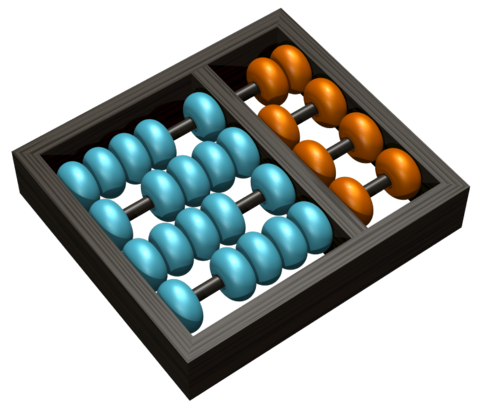
\includegraphics[width=0.25\textwidth]{imagens/Logo}\\
        \vspace{1.5cm}
        \Huge
    	\textbf{MO443 - Introdução ao Processamento de Imagem Digital}\\
        \vspace{0.5cm}
        \textbf{Relatório 1}\\
        \vspace{0.5cm}
        \Large
        \textbf{Aluno}: Julio Vinicius Amaral Oliveira\\
        \textbf{RA}: 230537\\
        \vspace{1.2cm}
    	\Large 
    	Instituto de Computação\\
    	Universidade Estadual de Campinas\\
    	\vspace{1.5cm}
        Campinas, 07 de Abril de 2025.
    \end{center}
\end{titlepage}
\tableofcontents
\clearpage

\newcommand{\shellcmd}[1]{\texttt{\footnotesize\# #1}}%estilizando citação de comandos do shell

\section{Introdução} 
O seguinte trabalho visa mostrar a aplicação de técnicas iniciais de processamento de imagem digital. Tais como conversão de cores, filtragem utilizando máscaras, manipulação de imagens como espelhamento. Essas técnicas são importantes para formar o alicerce teórico e prático que será utilizado ao longo de todas as técnicas futuras de processamento de imagem. Ao longo do trabalho, mostraremos como os desafios propostos foram resolvidos, além de justificar as escolhas tomadas e problemas enfrentados durante o desenvolvimento.
\section{Materiais e métodos}
Para resolução dos exercícios propostos, utilizamos as bibliotecas:
\begin{itemize}
    \item \texttt{OpenCV}: Utilizada para ler, processar e exibir imagens
    \item \texttt{Numpy}: Responsável pelo tratamento dos dados das imagens como arrays. É usada para realizar operações matemáticas e manipulação dos pixels de forma vetorizada, fundamental para o processamento de imagens de forma performática
    \item \texttt{scipy}: Foi utilizada apenas a função \texttt{convolve2d} que aplica operações de convolução em imagens de forma a implementar os filtros de extração de bordas e aprimoramento de detalhes
    \item \texttt{matplotlib}: Utilizado para a visualização das imagens no ambiente do Jupyter Notebook
    
\end{itemize}
\section{Códigos auxiliares}
Para a resolução dos desafios propostos, criamos uma série de códigos auxiliares que serviram para encapsular a lógica de uma sequência de comandos. Os códigos auxiliares criados foram:

\begin{lstlisting}[language=Python, caption={Funções auxiliares para visualização de imagens}]
def show_image_in_window(image):
    cv2.imshow('image', image)
    cv2.waitKey(0)
    cv2.destroyAllWindows()

def print_mono_image(image):
    plt.imshow(image, cmap='gray')
    plt.axis('off')
    plt.show()
    
def print_image(image):
    plt.imshow(image)
    plt.axis('off')
    plt.show()
\end{lstlisting}

A função \texttt{show\_image\_in\_window} serve para o OpenCV abrir uma imagem em uma tela separada, assim podemos verificar qual foi a imagem gerada. Além disso, temos a função \texttt{print\_mono\_image} que possibilita vermos a imagem sendo gerada no próprio Jupyter Notebook para imagens monocromáticas, e a função \texttt{print\_image} para imagens coloridas, facilitando também o trabalho de correção.

Durante o desenvolvimento, a função \texttt{show\_image\_in\_window} foi mais utilizada pois não havia necessidade das imagens ficarem como output de código o tempo todo, porém para a versão final do código, modificamos todas as suas chamadas para funções de visualização no notebook, como a \texttt{print\_mono\_image} e \texttt{print\_image}, conforme apropriado para cada tipo de imagem.

\section{Exercícios e discussão}
\subsection{Exercício 1: Esboço a lápis}
\paragraph{Objetivo:} 
Transformar uma imagem colorida em um esboço a lápis por meio da conversão para tons de cinza, aplicação de blur gaussiano e divisão pixel a pixel.

\paragraph{Estratégia:} 
Carregamos a imagem e convertemos para tons de cinza utilizando \texttt{cv2.cvtColor}. Em seguida, aplicamos um blur gaussiano com kernel de tamanho \texttt{(21, 21)} e \texttt{sigmaX = sigmaY = 0}, o que deixa o OpenCV calcular o sigma automaticamente. Para realçar os contornos, usamos a função \texttt{cv2.divide} dividindo a imagem original em tons de cinza por sua versão desfocada.

\paragraph{Discussão:} 
A divisão sugerida no enunciado da questão tinha como objetivo tornar mais claras regiões em que o 
pixel\_blur < pixel\_mono resultam já que a divisão resultariam em um número maior que 1 e ao reescalarmos a divisão ficaria com um valor próximo do limite superior. Analogamente, o oposto aconteceria quando pixel\_blur > pixel\_mono, e essa última opção acontece principalmente em regiões de borda, já que o blur aumenta o valor dos pixels ao redor de uma borda ao aplicar uma média dos pixels ao redor.

\paragraph{Resultado:} 
A imagem resultante se assemelha a um desenho a lápis, com destaque para as bordas e contornos principais.
\begin{figure}[H]
  \centering
  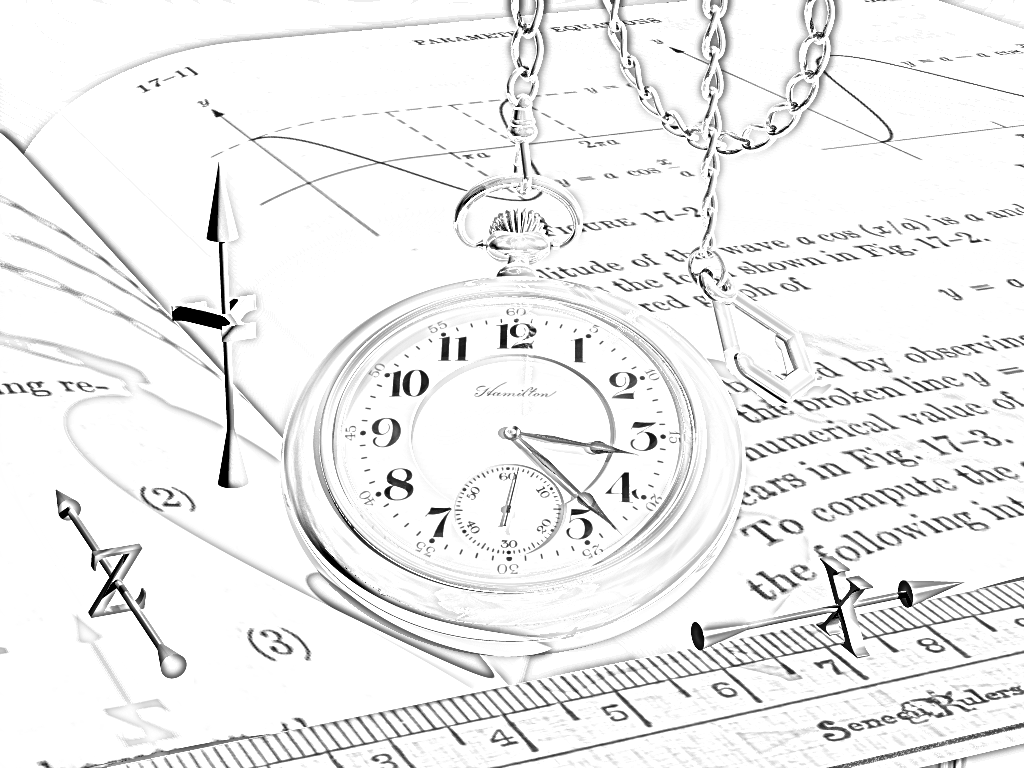
\includegraphics[width=0.4\textwidth]{imagens/ex1.png}
  \caption{Resultado do Exercício 1}
\end{figure}

\subsection{Exercício 2: Ajuste de brilho}
\paragraph{Objetivo:} 
Ajustar o brilho de uma imagem monocromática utilizando correção gama com diferentes valores de \( \gamma \).

\paragraph{Estratégia:} 
Primeiramente, carregamos a imagem monocromática e normalizamos os valores de pixel para o intervalo \texttt{[0, 1]}. Depois, aplicamos a transformação gama com \texttt{np.power} usando o valor \texttt{gamma = 3.5}. Após isso, reescalamos os valores de volta para o intervalo \texttt{[0, 255]}.

\paragraph{Discussão:} 
O uso do \texttt{np.power} para aplicar a transformação \( A^{1/\gamma} \) permite ajustar a percepção de brilho de forma não linear de forma vetorizada, contribuindo para performance da operação. Valores de gamma maiores que 1 clareiam a imagem pois sua operação semelhante a aplicar uma raiz de \(\gamma \) em um número entre 0 e 1, que causa o aumento desse número, e a normalização garante que os pixels estejam corretamente escalados antes e depois da transformação.


\paragraph{Resultado:} 
Imagens mais claras ou mais escuras, dependendo do valor de \( \gamma \), evidenciam diferentes aspectos da cena.
\begin{figure}[H]
    \centering
    \begin{subfigure}[b]{0.3\textwidth}
        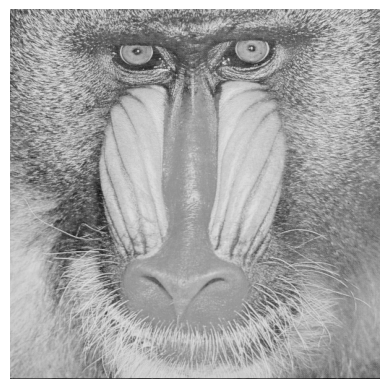
\includegraphics[width=\textwidth]{imagens/ex2-1.png}
        \caption{Para \( \gamma \) = 1.5 }
    \end{subfigure}
    \hfill
    \begin{subfigure}[b]{0.3\textwidth}
        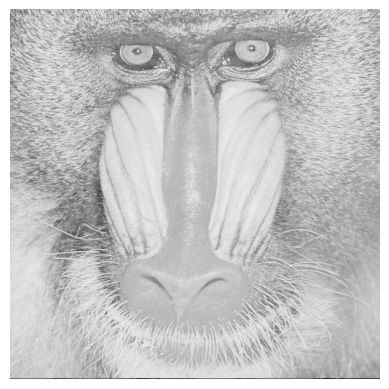
\includegraphics[width=\textwidth]{imagens/ex2-2.png}
        \caption{Para \( \gamma \) = 2.5 }
    \end{subfigure}
    \hfill
    \begin{subfigure}[b]{0.3\textwidth}
        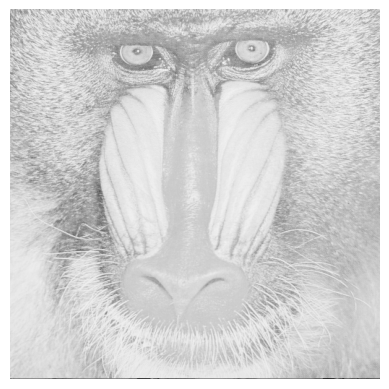
\includegraphics[width=\textwidth]{imagens/ex2-3.png}
        \caption{Para \( \gamma \) = 3.5 }
    \end{subfigure}
    \caption{Resultado do exercício 2}
\end{figure}


\subsection{Exercício 3: Mosaico}
\paragraph{Objetivo:} 
Reorganizar blocos de uma imagem monocromática segundo uma nova ordem específica, formando um mosaico.

\paragraph{Estratégia:} 
Carregamos a imagem e dividimos em blocos 4×4. Em seguida, usamos um dicionário (\texttt{image\_blocks\_mapper}) para mapear a posição original de cada bloco para uma nova posição para que então eu utilizasse um novo dicionário que mapeasse as mesmas posições mas agora como índices de uma matriz (Ex: posição 2 da matriz original viraria uma tupla (0, 1)), o algoritmo usado para realizar o mapeamento está descrito abaixo, trata-se de um algoritmo simples que acha o valor da coluna ao obter o valor do resto do indice pelo tamanho do bloco e o valor da linha pelo valor da sua divisão inteira. Por fim, utilizei slicing com NumPy para copiar os blocos da imagem original para suas novas posições na imagem final. 
\begin{lstlisting}[language=Python, caption={Algoritmo para encontrar index de linhas e colunas}]
def get_pos_from_coords(pos):
    row = (pos - 1) // block_size
    column = (pos - 1) % block_size
    return row, column

\end{lstlisting}

\paragraph{Discussão:} 
O uso de slicing com mapeamento via dicionário permitiu reorganizar os blocos de forma clara. Durante o desenvolvimento, também precisei criar uma nova matriz para colocar os pixels embaralhados, já que percebi que não era possível usar a mesma matriz através do algoritmo escolhido por mim, já que da forma que foi pensada ao mapearmos, por exemplo, a posição 1 da matriz da esquerda na posição 1 da matriz da direita, perdíamos a informação do número anterior que fora substituído. Segue abaixo o algoritmo que fez a reordenação, sendo h a altura e w a largura da imagem:
\begin{lstlisting}[language=Python, caption={Algoritmo de slicing utilizado}]
for left_coord, right_coord in coords_mapper.items():
    left_row, left_column = left_coord[0] , left_coord[1] 
    right_row, right_column = right_coord[0] , right_coord[1] 
    result_img[left_row * h: (left_row + 1) * h, left_column * w: (left_column + 1) * w ] = image[right_row * h: (right_row + 1) * h, right_column * w: (right_column + 1) * w ]

\end{lstlisting}

\paragraph{Resultado:} 
A imagem final apresenta um rearranjo dos blocos.
\begin{figure}[H]
  \centering
  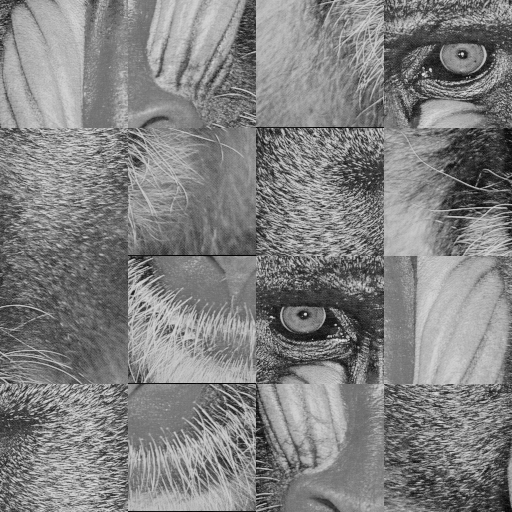
\includegraphics[width=0.4\textwidth]{imagens/ex3.png}
  \caption{Resultado do rearranjo dos blocos}
\end{figure}

\subsection{Exercício 4: Alteração de cores}
\paragraph{Objetivo:} 
Aplicar uma transformação linear nos canais RGB para simular o efeito de fotografias antigas.

\paragraph{Estratégia:} 
Convertemos a imagem de BGR para RGB, e aplicamos uma multiplicação matricial entre cada pixel e a matriz de transformação sugerida. A matriz foi transposta (\texttt{M.transpose()}) para alinhar corretamente com os vetores de cores. O resultado foi limitado ao intervalo \texttt{[0, 255]} e convertido para \texttt{uint8}.

\paragraph{Discussão:} 
A conversão foi necessária para que durante a multiplicação de matrizes os canais fossem multiplicados de forma correta, foi usado o operador np.matmul() para que a operação fosse vetorizada e também a imagem foi clipada para que os valores não ultrapassem 255.

\paragraph{Resultado:} 
A imagem adquire tonalidades amareladas, características de fotos envelhecidas.
\begin{figure}[H]
  \centering
  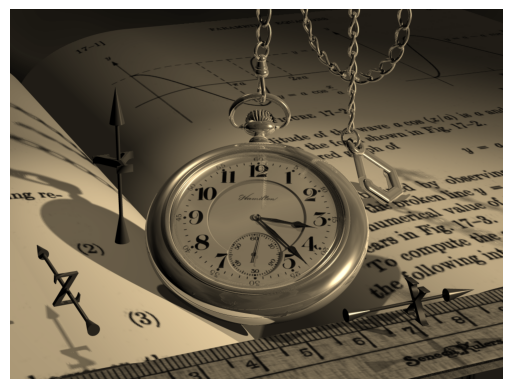
\includegraphics[width=0.4\textwidth]{imagens/ex4.png}
  \caption{Imagem envelhecida}
\end{figure}

\subsection{Exercício 5: Transformação de imagens coloridas}
\paragraph{Objetivo:} 
Aplicar duas transformações: uma linear nos canais RGB e outra para gerar uma imagem com uma única banda de cor baseada em média ponderada.

\paragraph{Estratégia:} 
Para a primeira parte, reaproveitamos a transformação linear feita no exercício anterior. Na segunda parte, utilizamos uma matriz 1×3 com os pesos de luminância (0.2989, 0.5870, 0.1140) e aplicamos sobre a imagem RGB usando multiplicação matricial, gerando uma imagem com apenas uma banda de cor.

\paragraph{Discussão:} 
A primeira transformação altera a imagem de forma estética (efeito sépia). Já a segunda transformação, baseada na média ponderada de canais RGB, é uma conversão para tons de cinza. Um desafio técnico encontrado foi a incompatibilidade entre as ordens dos canais esperadas pelo OpenCV (BGR) e pelo Matplotlib (RGB). Para mostrar corretamente a imagem processada, foi preciso reconverter o resultado utilizando \texttt{cv2.cvtColor()} com o parâmetro \texttt{cv2.COLOR\_RGB2BGR} antes da visualização, conforme evidenciado pela comparação na \autoref{fig:ex5_rgb}, onde a ausência dessa reconversão resultava em canais trocados.


\paragraph{Resultado:} 
Obtivemos imagens estilizadas ou com intensidade baseada na luminância.
\begin{figure}[H]
    \centering
    \begin{subfigure}[b]{0.3\textwidth}
        \includegraphics[width=\textwidth]{imagens/ex5-a.png}
        \caption{Resultado item A }
    \end{subfigure}
    \hfill
    \begin{subfigure}[b]{0.3\textwidth}
        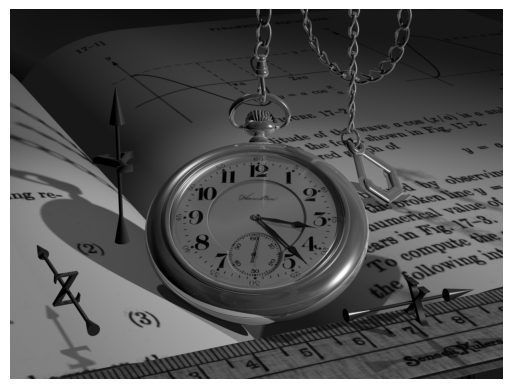
\includegraphics[width=\textwidth]{imagens/ex5-b.png}
        \caption{Resultado item B}
    \end{subfigure}
    \hfill
    \begin{subfigure}[b]{0.3\textwidth}
        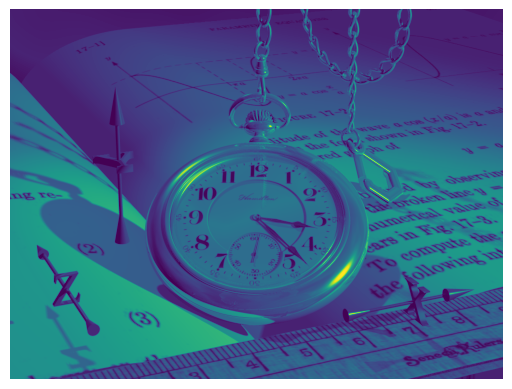
\includegraphics[width=\textwidth]{imagens/ex5-rgb.png}
        \caption{Item B RGB}
        \label{fig:ex5_rgb}
    \end{subfigure}
    \caption{Resultado do exercício 5}
\end{figure}


\subsection{Exercício 6: Planos de bits}
\paragraph{Objetivo:} 
Extrair os planos de bits de uma imagem monocromática.

\paragraph{Estratégia:} 
Utilizamos operações bit a bit (\texttt{<<}, \texttt{\&}, \texttt{>>}) para extrair planos de bits específicos da imagem. Para cada plano, criamos uma máscara com \texttt{1 << bit\_index}, aplicamos \texttt{bitwise\_and}, depois deslocamos os bits para a direita e multiplicamos por 255 para exibir o plano como imagem.

\paragraph{Discussão:} 
Esse método permite extrair de forma performática os bits que compõem os valores de intensidade da imagem. A visualização de cada plano ajuda a entender como diferentes bits afetam a representação visual da imagem, bits mais significativos, tendem a se parecer mais com a imagem original, já bits menos significativos só nos mostram um ruído.
\begin{lstlisting}[language=Python, caption={Função utilizada para extração de bits}]
def extract_bit(bit_index):
    bit_mask = 1 << bit_index 
    extracted_bits  = np.bitwise_and(image, bit_mask) #Gera um valor como 00100000
    normalized_bit_image = extracted_bits  >> bit_index # Converte os valores como 00000000 ou 00100000 para 0 ou 1
    return normalized_bit_image * 255
\end{lstlisting}

\paragraph{Resultado:} 
Planos inferiores contêm mais ruído, enquanto os superiores preservam a estrutura principal da imagem.
\begin{figure}[H]
    \centering
    \begin{subfigure}[b]{0.32\textwidth}
        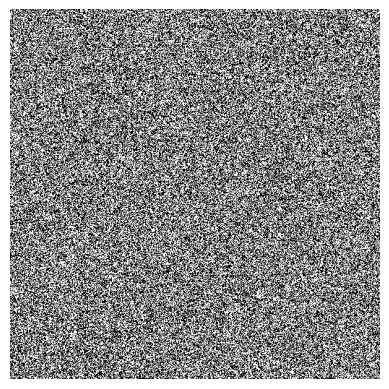
\includegraphics[width=\textwidth]{imagens/ex6-0.png}
        \caption{Plano de bits ordem 0}
    \end{subfigure}
    \hfill
    \begin{subfigure}[b]{0.32\textwidth}
        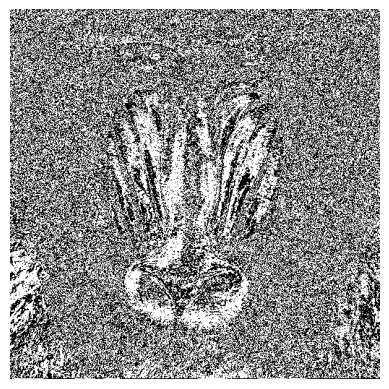
\includegraphics[width=\textwidth]{imagens/ex6-4.png}
        \caption{Plano de bits ordem 4}
    \end{subfigure}
    \hfill
    \begin{subfigure}[b]{0.32\textwidth}
        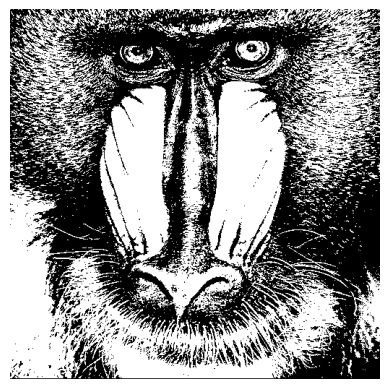
\includegraphics[width=\textwidth]{imagens/ex6-7.png}
        \caption{Plano de bits ordem 7}
    \end{subfigure}
    \caption{Resultado do exercício 6}
\end{figure}


\subsection{Exercício 7: Combinação de imagens}
\paragraph{Objetivo:} 
Combinar duas imagens monocromáticas por meio de média ponderada.

\paragraph{Estratégia:} 
Carregamos duas imagens monocromáticas (\texttt{baboon} e \texttt{butterfly}) e convertemos para \texttt{float32}. Utilizamos multiplicação escalar com os pesos \texttt{\(\alpha\)} e \texttt{\(\beta\)}, em seguida somamos os resultados com \texttt{np.add}. A imagem final foi normalizada para o intervalo \texttt{[0, 255]} com \texttt{np.clip} e convertida para \texttt{uint8}.

\paragraph{Discussão:} 
A utilização dessa estratégia foi bem direta, só precisamos ter que tomar cuidado para não realizar operações de forma escalar, por isso usamos o \texttt{np.multiply} e o \texttt{np.add} para garantir a vetorização das operações.

\paragraph{Resultado:} 
A imagem resultante apresenta uma mistura entre as duas imagens originais.
\begin{figure}[H]
    \centering
    \begin{subfigure}[b]{0.32\textwidth}
        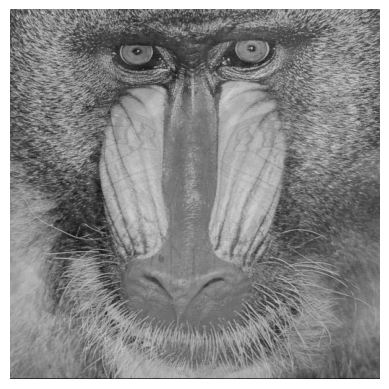
\includegraphics[width=\textwidth]{imagens/ex7-1.png}
        \caption{\(\alpha\)=0.8 e \(\beta\) = 0.2}
    \end{subfigure}
    \hfill
    \begin{subfigure}[b]{0.32\textwidth}
        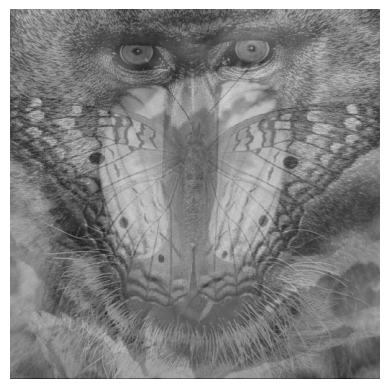
\includegraphics[width=\textwidth]{imagens/ex7-2.png}
        \caption{\(\alpha\)=0.5 e \(\beta\) = 0.5}
    \end{subfigure}
    \hfill
    \begin{subfigure}[b]{0.32\textwidth}
        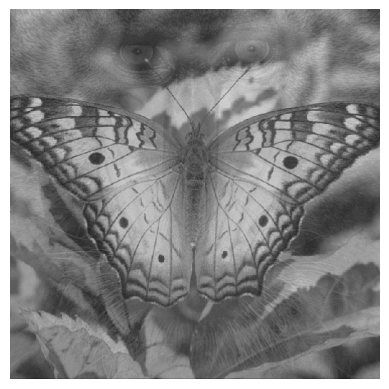
\includegraphics[width=\textwidth]{imagens/ex7-3.png}
        \caption{\(\alpha\)=0.2 e \(\beta\) = 0.8}
    \end{subfigure}
    \caption{Resultado do exercício 7}
\end{figure}

\subsection{Exercício 8: Transformação de intensidade}
\paragraph{Objetivo:} 
Aplicar diferentes transformações nos níveis de cinza da imagem, como negativo, mapeamento de intervalo e espelhamento.

\paragraph{Estratégia:} 
Implementamos diversas transformações sobre uma imagem monocromática:
\begin{itemize}
  \item (a) Inversão dos tons com \texttt{np.negative}.
  \item (b) Aplicação de transformação linear com a equação $g = \frac{20 \cdot f + 5100}{51}$.
  \item (c) Inversão horizontal de linhas pares com slicing \texttt{img[::2] = img[::2, ::-1]}.
  \item (d) Espelhamento vertical da metade inferior da imagem com slicing reverso.
  \item (e) Espelhamento total da imagem, invertendo todas as linhas.
\end{itemize}

\paragraph{Discussão:} 
\begin{itemize}
  \item (a) Para o item A, não houve nenhum desafio muito grande, a aplicação direta do \texttt{np.negative} já retornou a imagem esperada
  \item (b) Para o item B, foi feito uma regra de proporcionalidade simples para chegarmos na equação $g = \frac{20 \cdot f + 5100}{51}$, em que f é a imagem original e g sua imagem transformada. Entretanto, não tivemos sucesso em obter a imagem proposta pelo exercício, a imagem ficou com aspecto de lavada e não com o aspecto escuro assim como o exercício sugeriu.
  \item (c) Para o item C, fizemos apenas uma manipulação simples usando slicing \texttt{img[::2] = img[::2, ::-1]}.
  \item (d) Para o item D, realizamos uma atribuição onde a segunda metade do array img (\texttt{img[w//2:w]}) recebe os valores da primeira metade (\texttt{img[w//2:0:-1]}) em ordem reversa, criando um espelhamento horizontal
  \item (e) Para o item E, fizemos com que a imagem recebesse sua versão revertida com o comando \texttt{img = img[w:0:-1]}
\end{itemize}
\paragraph{Resultado:} 
Obtivemos imagens modificadas com efeitos visuais distintos, como inversão de direção e simetria.
\begin{figure}[H]
  \centering
  \begin{subfigure}{0.3\textwidth}
    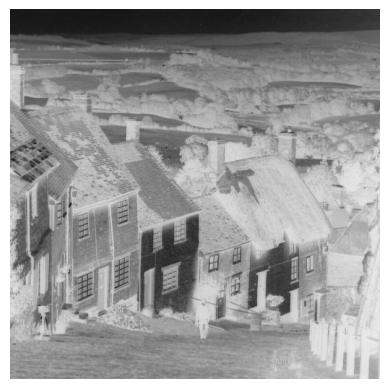
\includegraphics[width=\linewidth]{imagens/ex8-a.png}
    \caption{Item A}
  \end{subfigure}
  \begin{subfigure}{0.3\textwidth}
    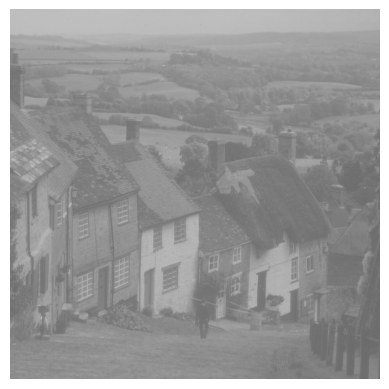
\includegraphics[width=\linewidth]{imagens/ex8-b.png}
    \caption{Item B}
  \end{subfigure}
  \begin{subfigure}{0.3\textwidth}
    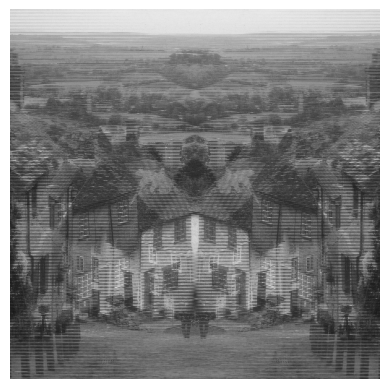
\includegraphics[width=\linewidth]{imagens/ex8-c.png}
    \caption{Item C}
  \end{subfigure}

  \begin{subfigure}{0.3\textwidth}
    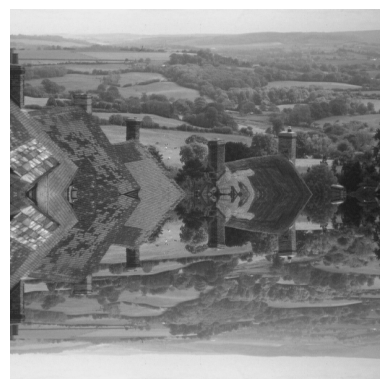
\includegraphics[width=\linewidth]{imagens/ex8-d.png}
    \caption{Item D}
  \end{subfigure}
  \begin{subfigure}{0.3\textwidth}
    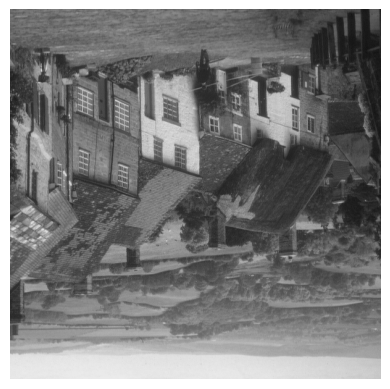
\includegraphics[width=\linewidth]{imagens/ex8-e.png}
    \caption{Item E}
  \end{subfigure}

  \caption{Resultados Exercício 8}
\end{figure}

\subsection{Exercício 9: Quantização de imagens}
\paragraph{Objetivo:} 
Reduzir o número de níveis de cinza usados para representar uma imagem.

\paragraph{Estratégia:} 
Aplicamos a quantização reduzindo os níveis de cinza para múltiplos de $k$, onde $k = \frac{256}{n}$, com $n$ sendo os níveis desejados, depois reescalamos a imagem multiplicando por k. A expressão ficou então: 
\[
\left\lfloor \frac{\text{img}}{k} \right\rfloor \cdot k
\].

\paragraph{Discussão:} 
Neste exercício, embora a solução adotada pareça simples, envolvendo apenas uma multiplicação e uma divisão, conseguimos resultados visuais muito próximos das imagens fornecidas no PDF.

No entanto, ao reduzir para o \textbf{nível 2}, enfrentamos um comportamento inesperado na geração da imagem. Esperávamos que o algoritmo aplicasse uma \textbf{binarização clássica}, como:

\begin{align*}
\text{Se } x < 128 &\Rightarrow 0 \quad \text{(preto)} \\
\text{Se } x \geq 128 &\Rightarrow 255 \quad \text{(branco)}
\end{align*}

Mas o que ocorreu foi:

\begin{align*}
  \text{Se } x < 128 &\Rightarrow 0 \quad \text{(preto)} \\
  \text{Se } x \geq 128 &\Rightarrow 128 \quad \text{(cinza escuro)}
\end{align*}

Isso gerou uma imagem com tons mais escuros, ao invés do contraste marcado entre preto e branco.


\begin{lstlisting}[language=Python, caption={Algoritmo utilizado para quantização das imagens}]
def quantize(img, n):
    k = 256 // n
    return (img // k) * k
\end{lstlisting}

\paragraph{Resultado:} 
A imagem perde gradativamente detalhes e suavidade à medida que os níveis diminuem.
\begin{figure}[H]
  \centering
  \begin{subfigure}{0.3\textwidth}
    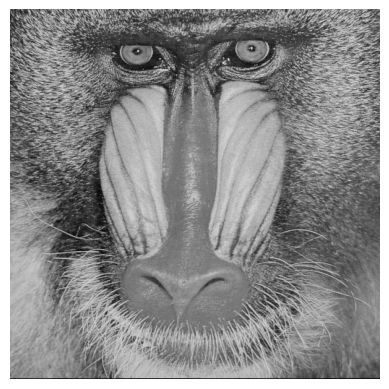
\includegraphics[width=\linewidth]{imagens/ex9-1.png}
    \caption{256 níveis}
  \end{subfigure}
 \begin{subfigure}{0.3\textwidth}
    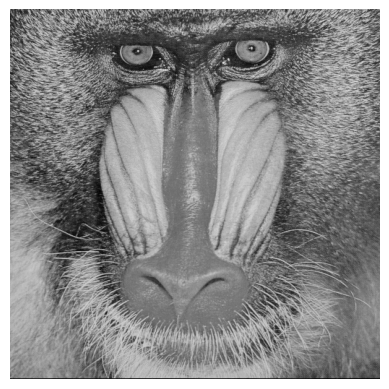
\includegraphics[width=\linewidth]{imagens/ex9-2.png}
    \caption{64 níveis}
  \end{subfigure}
  \begin{subfigure}{0.3\textwidth}
    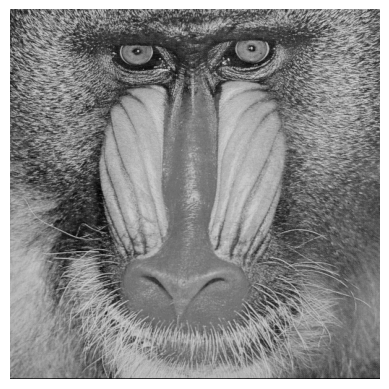
\includegraphics[width=\linewidth]{imagens/ex9-3.png}
    \caption{32 níveis}
  \end{subfigure}
  \begin{subfigure}{0.3\textwidth}
    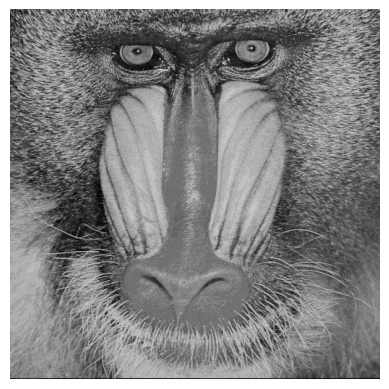
\includegraphics[width=\linewidth]{imagens/ex9-4.png}
    \caption{16 níveis}
  \end{subfigure}
  \begin{subfigure}{0.3\textwidth}
    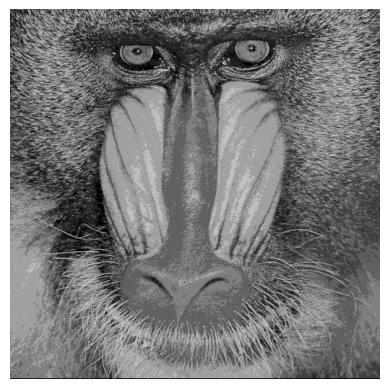
\includegraphics[width=\linewidth]{imagens/ex9-5.png}
    \caption{8 níveis}
  \end{subfigure}
  \begin{subfigure}{0.3\textwidth}
    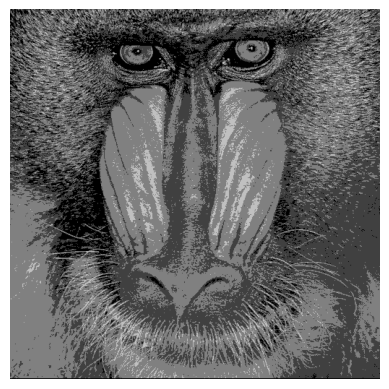
\includegraphics[width=\linewidth]{imagens/ex9-6.png}
    \caption{4 níveis}
  \end{subfigure}
  \begin{subfigure}{0.3\textwidth}
    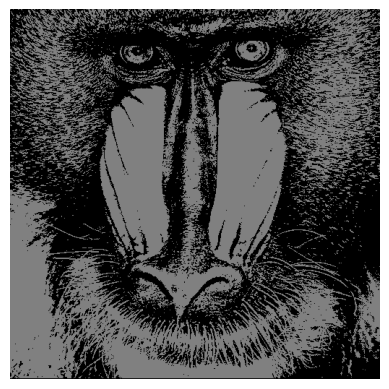
\includegraphics[width=\linewidth]{imagens/ex9-7.png}
    \caption{2 níveis}
  \end{subfigure}
  \caption{Resultados Exercício 9}
\end{figure}

\subsection{Exercício 10: Filtragem de imagens}
\paragraph{Objetivo:} 
Aplicar filtros espaciais sobre uma imagem monocromática, utilizando operações de convolução com máscaras definidas previamente. O objetivo é observar os diferentes efeitos produzidos pelos filtros sobre a imagem original, como realce de bordas, suavização e detecção de padrões.

\paragraph{Estratégia:} 
Foi utilizada convolução 2D entre a imagem de entrada e as máscaras fornecidas. Cada filtro foi aplicado individualmente, exceto os filtros $h_3$ e $h_4$, que também foram combinados de acordo com a fórmula:
\[
\text{resultado} = \sqrt{(h_3)^2 + (h_4)^2}
\]
A função `convolve2d` do pacote \texttt{scipy.signal} foi utilizada com o modo de borda `'same'` para preservar o tamanho da imagem original. Os resultados foram normalizados para o intervalo $[0, 255]$ .
Dado a natureza repetitiva da solução, optamos por criar uma função que recebia o kernel e o caminho da imagem original, retornando depois a imagem transformada, sendo ela:

\begin{lstlisting}[language=Python, caption={Algoritmo utilizado para quantização das imagens}]
def apply_filter(kernel, image):
    convolved_image = convolve2d(image, kernel, mode='same', boundary='fill', fillvalue=0)
    clipped_image = np.clip(convolved_image, 0, 255)
    print_mono_image(clipped_image.astype(np.uint8))
    return clipped_image
\end{lstlisting}

\paragraph{Discussão:} 
A seguir descrevemos os efeitos observados com cada filtro:

\begin{enumerate}
    \item \textbf{Filtro $h_1$}: Destaca fortemente os contornos da imagem, fazendo com que nós percebamos nitidamente, a imagem escolhida para mostrar isso é a da cidade em que é possível ver o desenho de todas as casas
    \begin{figure}[H]
      \centering
      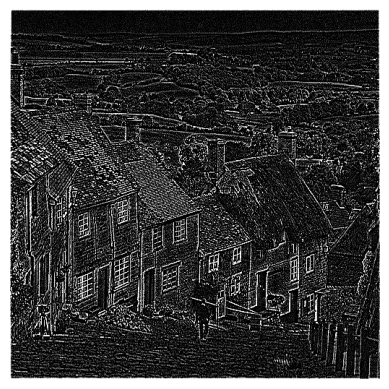
\includegraphics[width=0.6\textwidth]{imagens/ex10-01.png}
      \caption{Filtro $h_1$}
    \end{figure}
    \item \textbf{Filtro $h_2$}: Este filtro aplica um blur gaussiano 5x5, suavizando a imagem. Comparando a imagem original na \autoref{fig:train_original_h2} com o resultado após a aplicação do filtro na \autoref{fig:train_blur_h2}, podemos observar claramente a perda de nitidez.
    \begin{figure}[H]
      \centering
      \begin{subfigure}{0.8\textwidth}
        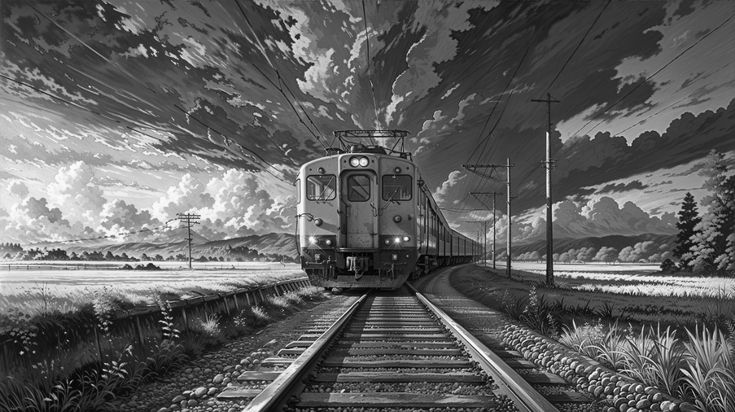
\includegraphics[width=\linewidth]{imagens/train_original.png}
        \caption{Imagem original de um trem}
        \label{fig:train_original_h2}
      \end{subfigure}
      \begin{subfigure}{0.8\textwidth}
        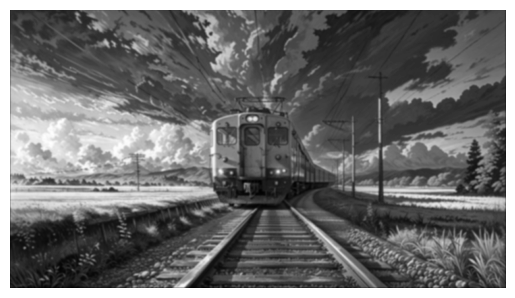
\includegraphics[width=\linewidth]{imagens/train_blur.png}
        \caption{Imagem após filtro $h_2$}
        \label{fig:train_blur_h2}
      \end{subfigure}
    \end{figure}
    \item \textbf{Filtro $h_3$}: Este filtro realça bordas verticais. Para verificar isso, utilizamos a imagem \autoref{fig:imagem_gerada_artificialmente}, gerada através de inteligência artificial, que tem elementos bem simples mas que tornam a visualização da funcionalidade do filtro clara. A \autoref{fig:realce_bordas_verticais} mostra o filtro marcando apenas as bordas verticais
    \begin{figure}[H]
      \centering
      \begin{subfigure}{0.8\textwidth}
        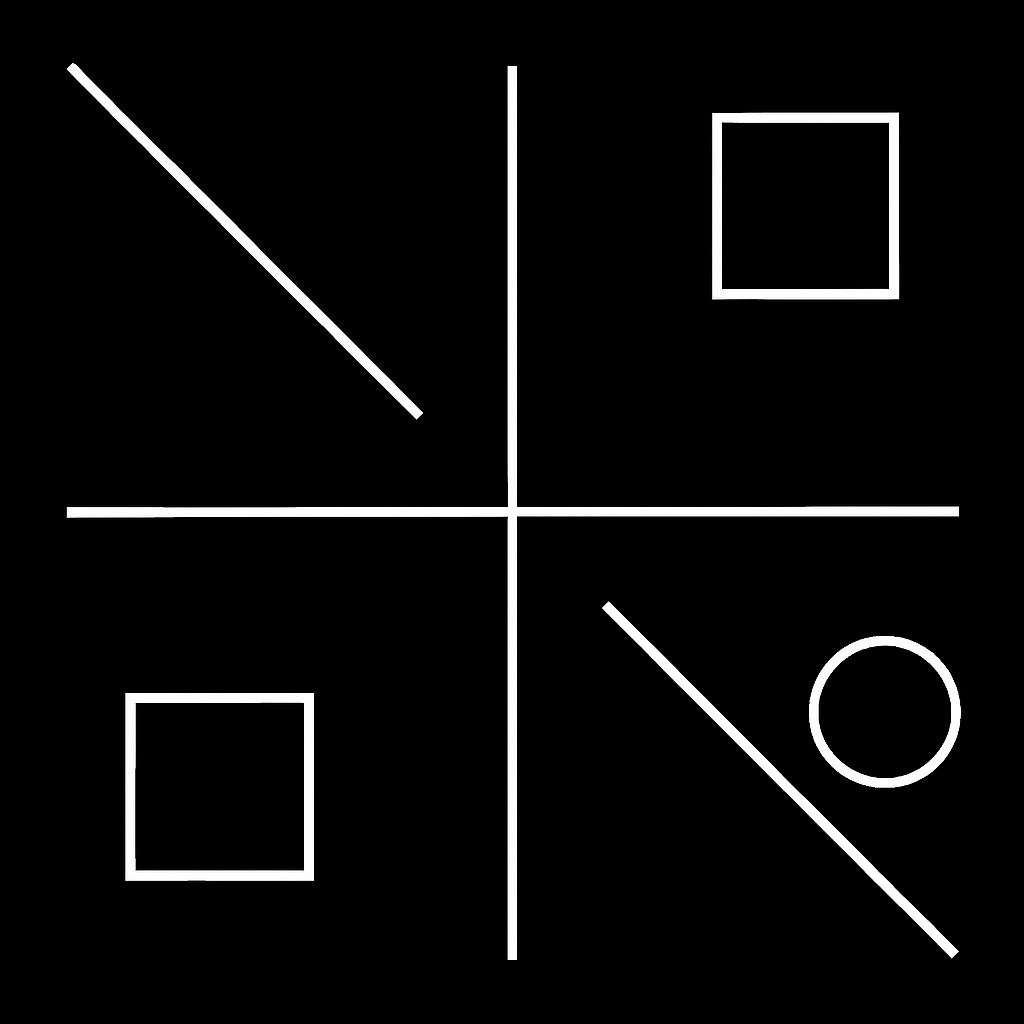
\includegraphics[width=\linewidth]{imagens/imagem_gerada_artificialmente.png}
      \caption{Imagem original gerada artificialmente}
      \label{fig:imagem_gerada_artificialmente}
      \end{subfigure}
      \begin{subfigure}{0.8\textwidth}
        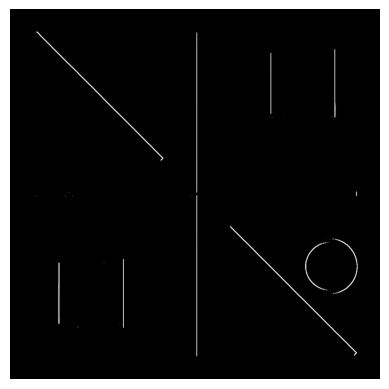
\includegraphics[width=\linewidth]{imagens/ex10-03.png}
        \caption{Imagem após filtro $h_3$}
        \label{fig:realce_bordas_verticais}
      \end{subfigure}
    \end{figure}
  
    \item \textbf{Filtro $h_4$}: Filtro que realça bordas horizontais, utilizando a mesma imagem que o exemplo anterior, podemos ver que agora o filtro está destacando os elementos horizontais da imagem
    \begin{figure}[H]
      \centering
      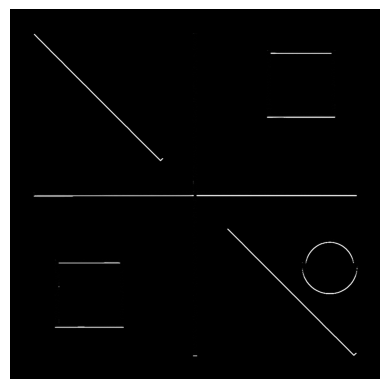
\includegraphics[width=0.6\textwidth]{imagens/ex10-04.png}
      \caption{Filtro $h_4$}
    \end{figure}
    \item \textbf{Combinação $h_3$ e $h_4$}: Utilizando a equação $\sqrt{(h_3)^2 + (h_4)^2}$ obtemos um resultado mais completo, esse filtro destaca os contornos em todas as direções. Podemos ver através da \autoref{fig:comb_h3_h4} que todos os contornos estão muito bem definidos
    \begin{figure}[H]
      \centering
      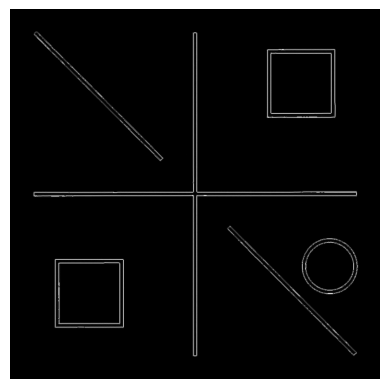
\includegraphics[width=0.6\textwidth]{imagens/ex10-03-04.png}
      \caption{Combinação $h_3$ e $h_4$}
      \label{fig:comb_h3_h4}
    \end{figure}
    \item \textbf{Filtro $h_5$}: Destaca o contorno da imagem, mas comparando com o filtro $h_1$, podemos notar que ele destaca mais fracamente esses contornos. É notório, por exemplo, que existe um contraste grande nos tijolos e telhados das casas ao utilizar o filtro $h_1$ e esse contraste exacerbado não é percebido usando o filtro $h_5$
    \begin{figure}[H]
      \centering
      \begin{subfigure}{0.6\textwidth}
        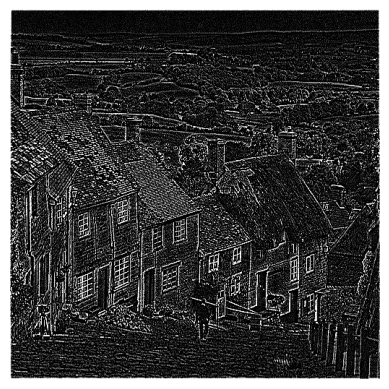
\includegraphics[width=\linewidth]{imagens/ex10-01.png}
      \caption{Imagem da cidade com filtro $h_1$}
      \end{subfigure}
      \begin{subfigure}{0.6\textwidth}
        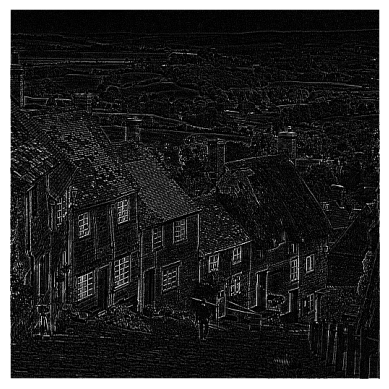
\includegraphics[width=\linewidth]{imagens/ex10-05.png}
        \caption{Imagem da cidade com filtro $h_5$}
      \end{subfigure}
    \end{figure}
    \item \textbf{Filtro $h_6$}: Gera um blur suave e reduz pequenos detalhes da imagem, podemos ver por exemplo, que na imagem com o filtro existem menos detalhes nas folhagens a esquerda, que são bem mais perceptíveis ao olhar a imagem original.
    \begin{figure}[H]
      \centering
      \begin{subfigure}{0.8\textwidth}
        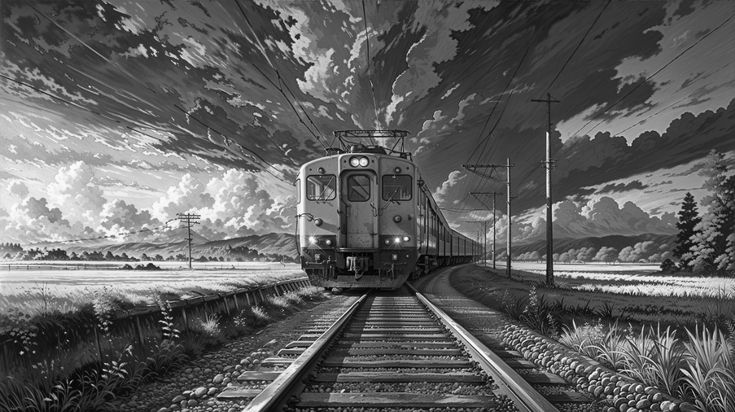
\includegraphics[width=\linewidth]{imagens/train_original.png}
        \caption{Imagem original de um trem}
      \end{subfigure}
      \begin{subfigure}{0.8\textwidth}
        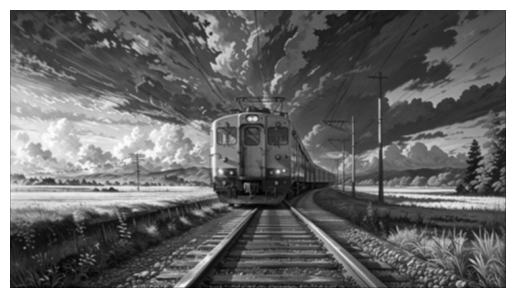
\includegraphics[width=\linewidth]{imagens/ex10-06.png}
        \caption{Imagem após filtro $h_6$}
      \end{subfigure}
    \end{figure}
    \item \textbf{Filtros $h_7$ e $h_8$}: Estes filtros detectam bordas diagonais, mas em direções opostas. O filtro $h_7$ destaca contornos na direção diagonal descendente ($\swarrow$ ), enquanto o filtro $h_8$ realça elementos na direção diagonal ascendente ($\nearrow$ ). Esta diferença fica evidente ao analisar os resultados: nas imagens processadas com $h_7$ (\autoref{fig:cidade_filtro_h7}), os contornos diagonais descendentes aparecem mais nítidos, enquanto com $h_8$ (\autoref{fig:cidade_filtro_h8}) os telhados e outras estruturas com inclinação ascendente ganham destaque.
    \begin{figure}[H]
      \centering
      \begin{subfigure}{0.6\textwidth}
        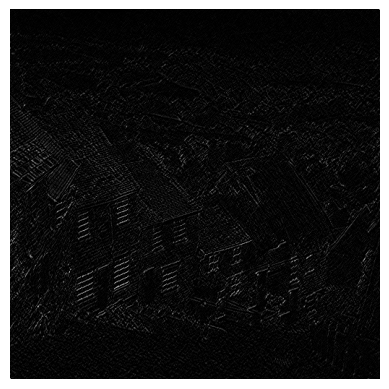
\includegraphics[width=\linewidth]{imagens/ex10-07.png}
        \caption{Imagem após filtro $h_7$}
        \label{fig:cidade_filtro_h7}
      \end{subfigure}
      \begin{subfigure}{0.6\textwidth}
        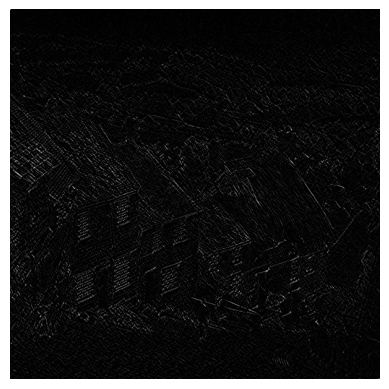
\includegraphics[width=\linewidth]{imagens/ex10-08.png}
        \caption{Imagem após filtro $h_8$}
        \label{fig:cidade_filtro_h8}
      \end{subfigure}
    \end{figure}
    \item \textbf{Filtro $h_9$}: Aplica um blur direcionado ao longo da diagonal descendente ($\nwarrow$ ). Analisando os resultados na imagem da Mona Lisa, observamos que os detalhes finos e texturas originais se transformam em listras diagonais, criando um efeito que ressalta essa direção específica.
    \begin{figure}[H]
      \centering
      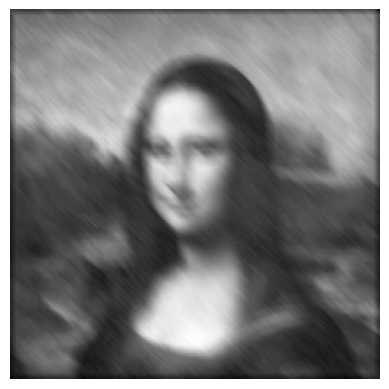
\includegraphics[width=0.6\textwidth]{imagens/ex10-09.png}
      \caption{Imagem após filtro $h_9$}
    \end{figure}
    \item \textbf{Filtro $h_{10}$}: Produz um efeito de realce de bordas, pode ser percebido, por exemplo, utilizando a imagem da casa, é notório que os tijolos da frente tem seus contornos mais marcados ao serem comparados com a imagem original.
    \begin{figure}[H]
      \centering
      \begin{subfigure}{0.6\textwidth}
        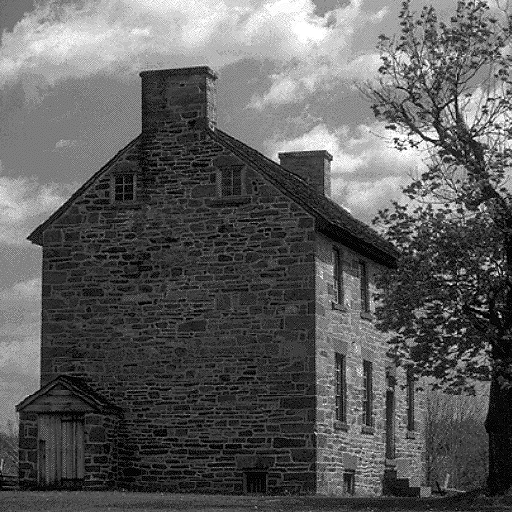
\includegraphics[width=\linewidth]{imagens/house.png}
        \caption{Imagem original da casa}
        \label{fig:house_original}
      \end{subfigure}
      \begin{subfigure}{0.6\textwidth}
        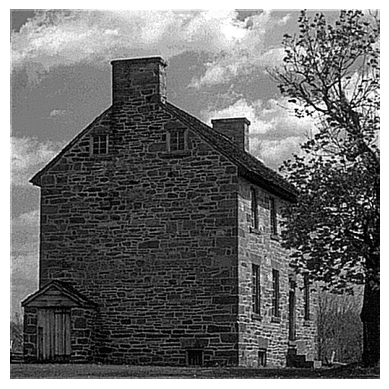
\includegraphics[width=\linewidth]{imagens/ex10-10.png}
        \caption{Imagem após filtro $h_{10}$}
        \label{fig:casa_filtro_h10}
      \end{subfigure}
    \end{figure}
    \item \textbf{Filtro $h_{11}$}: Realça bordas diagonais na direção ascendente ($\nearrow$). Na imagem do baboon monocromática, observamos que os pelos orientados nessa direção são significativamente destacados em comparação com pelos em outras orientações.
    \begin{figure}[H]
      \centering
      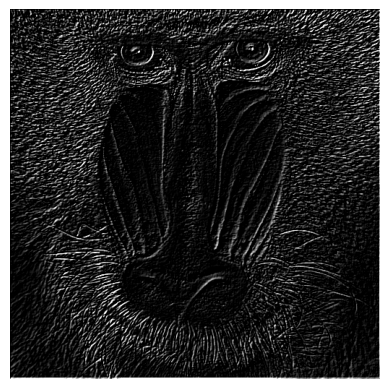
\includegraphics[width=0.6\textwidth]{imagens/ex10-11.png}
      \caption{Imagem após filtro $h_{11}$}
    \end{figure}
  \end{enumerate}

\end{document}